\documentclass{beamer}
\usetheme{CambridgeUS}

\title{Quantum City Challenge: Smart Charging of EVs}
\subtitle{Applying Quantum Technology in Alberta's Energy Industry}
\author{Quantum City}
\titlegraphic{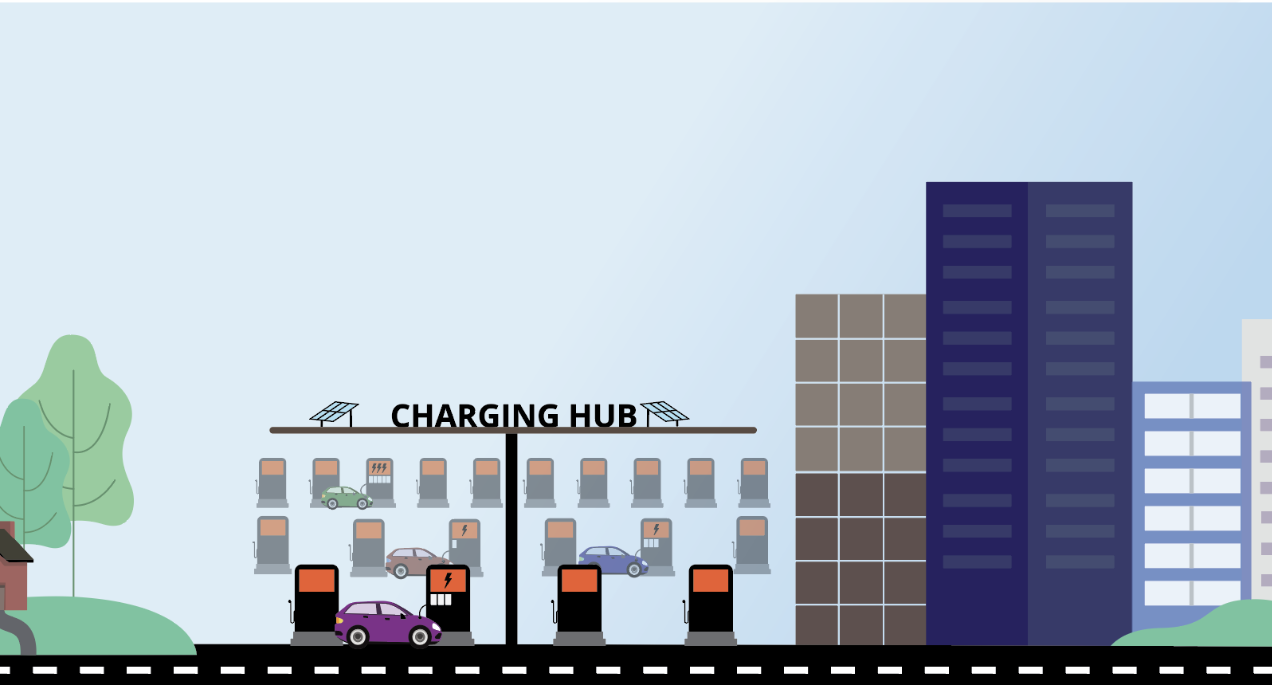
\includegraphics[width=0.5\linewidth]{Screenshot 2023-12-18 011307.png}}


\begin{document}

\begin{frame}
  \titlepage
\end{frame}


\begin{frame}
    \frametitle{The Demand}
    \begin{itemize}
        \pause
        \item Total EVs commuting: 25,000 with an average one-way commute time of 27.70 minutes.
        \pause
        \item Average EV efficiency: approximately 0.2 kWh per kilometer and an average speed of 50 km/h.
        \pause
        \item Daily two-way commute requires approximately 9.236 kWh per EV.
        \pause
        \item Average battery capacity: 50 kWh, requiring recharge every 5 days.
        \pause
        \item Daily charging needs: one-fifth of the commuters (5,000 EVs) 
        \pause
        \item We also account for  additional 2,000 EVs for minimal top-ups, totaling 7,000 EVs daily.
        \pause
        \item Maximum daily energy requirement: 7,000 EVs x 50 kWh = 350,000 kWh or 350 MWh.
    \end{itemize}
    \end{frame}
    
    \begin{frame}
    \frametitle{The Supply}
    \begin{itemize}
        \pause
        \item Charging hub: 30 stations, each with 100 Level 2 charging ports.
        \pause
        \item Level 2 charger capacity: up to 20 kW per port.
        \pause
        \item Consistent Voltage 240V with current varying between 0 and 64A
    \end{itemize}
    \end{frame}
    
    \begin{frame}{Objective}
       Suppose the average available charging time is:
       \begin{itemize}
        \item 6 hours for full charge on weekdays ( 4 hours on weekends)
        \item 1 hour for top-ups
       \end{itemize}
       \pause
       We must adjust the current of each charging port to ensure that every plugged-in  EV is served within the available
       charging time, while minimizing energy spending and without 
       exceeding the charging limits
       \begin{figure}
        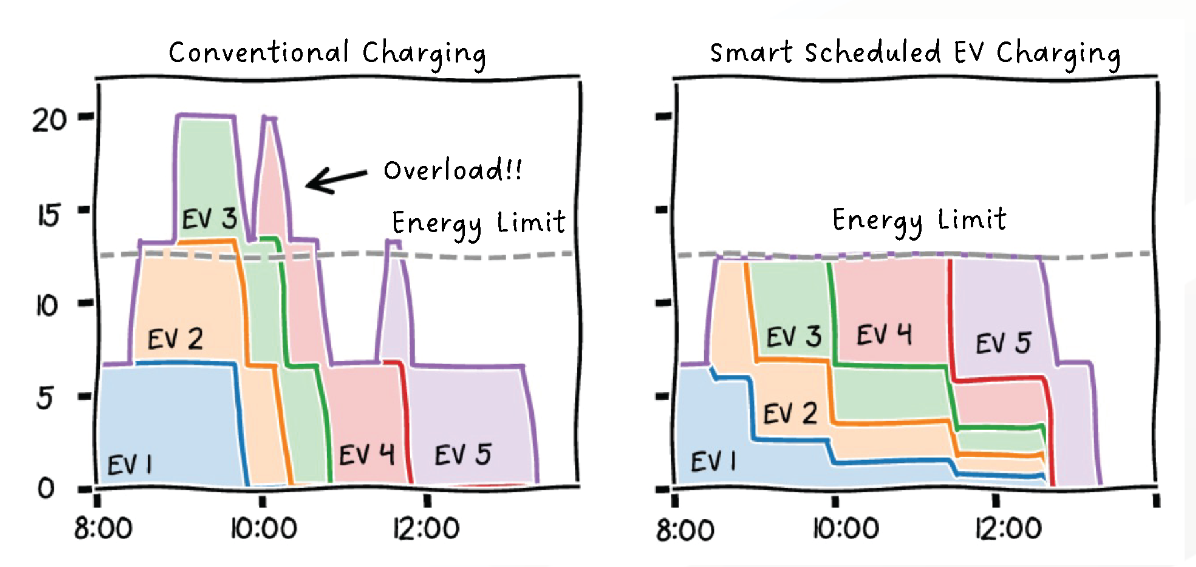
\includegraphics[width=0.7\linewidth]{Screenshot 2023-12-18 010917.png}
        \end{figure}
    \end{frame}

    \begin{frame}
    \frametitle{Mathematical Constraints}
    \begin{itemize}
        \pause
        \item Time is discrete into steps $\Delta t$ (15 or 30 minutes)
        \pause
        \item We define a horizon from $t_1$ to $T$ (6 to 12 hours)
        \pause
        \item $r_i(t_k)\in \rho$ is  the electric current at which the $i$th EV will be charged at time $t_k$, and $\rho = \{8,16,32,48,64\}A$
        \pause
        \item $e_i$ is the requested charge by $i$th EV. Thus
        $$e_i(t_k) = e_i - \sum_{j=0}^k r_i(t_j)*V*\Delta t$$
        \pause
        \item $v_{t_k}$ is a set that denotes the active EVs plugged-in at given $t_k$ (needs to be update in every time step)
        
    \end{itemize}
    \end{frame}

    \begin{frame}
    \frametitle{Mathematical Constraints}
    
        $$r_i(t_k)\in \rho \;\;\;if\;\;t_k\leq \tau_i^{end}\;\;\forall i \in v_{t_k}$$
        \pause
        $$r_i(t_k) = 0\;\;\; if\;\; t_k>\tau_i^{end}\;\;\;\forall i \in v_{t_k}$$
        \pause
        $$\sum_{j=0}^k r_i(t_j)\cdot V \cdot \Delta t \leq e_i(t_k)\;\;\;\forall i \in v_{t_k}$$
    
    \end{frame}


\begin{frame}
\frametitle{Cost Function}
$$U^{QC}(\hat{r}):= \sum_{k}\frac{T - t_k}{T-t_1}\sum_{i \in v_{t_k}} r_i(t_k)$$
$$U^{NC}(\hat{r}):=- \sqrt[p]{\sum_{i\in v_t}|\sum_{k}^{\tau^i_{end}} r_i(t_k)\cdot V\cdot \Delta - e_i|^p}$$
$$U^{LV}(\hat{r}):=-\sum_{k}\left(\sum_{i \in v_{t_k}} r_i(t_k)\right)^2$$
    %\sum_{i\in v_t} $$
\pause
$$U(\hat{r}) = \alpha U(\hat{r}) + \beta U^{NC}(\hat{r})+ \gamma U^{LV}(\hat{r})$$
\end{frame}



\end{document}
